% 174-21(174쪽) — 길이 6인 막대를 3등분 해 가운데를 버리는 시행을 두 번 한 모습(위: 처음 막대, 가운데: 1회 후 2개, 아래: 2회 후 4개).
% 스캔 그림이 흐려 TikZ 로 다시 그렸다. 라벨은 원문에 있는 6 만 두고 남은 길이(답)는 적지 않는다.
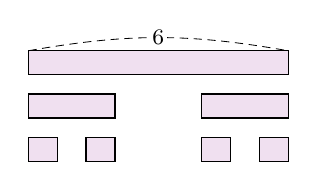
\begin{tikzpicture}[scale=0.55, line width=0.5pt]
  \draw[fill=violet!12] (0,2) rectangle (6,2.55);
  \draw[fill=violet!12] (0,1) rectangle (2,1.55);
  \draw[fill=violet!12] (4,1) rectangle (6,1.55);
  \draw[fill=violet!12] (0,0) rectangle (0.667,0.55);
  \draw[fill=violet!12] (1.333,0) rectangle (2,0.55);
  \draw[fill=violet!12] (4,0) rectangle (4.667,0.55);
  \draw[fill=violet!12] (5.333,0) rectangle (6,0.55);
  \draw[densely dashed, line width=0.3pt] (0,2.55)
    to[bend left=10] node[midway, fill=white, inner sep=1pt, font=\footnotesize] {$6$} (6,2.55);
\end{tikzpicture}
